\documentclass[pdf]{beamer}

\setbeamertemplate{caption}[numbered]

\usepackage{newfloat}

\usepackage{graphicx}
\usepackage{amsmath, amsthm, amssymb, amsfonts}
\usepackage{multicol}
\usepackage{multirow}
%\usepackage{fancyvrb}
%\fvset{fontsize=\normalsize}
\usepackage[inline]{enumitem}

\usepackage[newfloat]{minted}
\setminted{bgcolor=lightgray,fontsize=\normalsize,frame=leftline,linenos}
% \newmintinline[cinline]{c}{fontsize=\normalsize}
% \newmintinline[shinline]{sh}{fontsize=\normalsize,fgcolor=black}
\setmintedinline{bgcolor=lightgray,fontsize=\normalsize}

\usepackage[T1]{fontenc}
\usepackage[boldsans]{ccfonts}
\usepackage[euler-digits,euler-hat-accent]{eulervm}
\usepackage{cabin}
\usepackage[ activate={true,nocompatibility},final,tracking=true,%
  kerning=true,spacing=]{microtype}
\usepackage{inconsolata}
\setbeamertemplate{navigation symbols}{}

\renewcommand{\theFancyVerbLine}{\ttfamily {\footnotesize \arabic{FancyVerbLine}}}

\usepackage{enumitem}
\setlist[itemize,1]{label={\fontfamily{cmr}\fontencoding{T1}\selectfont\textbullet}}
\setlist[itemize,2]{label={\fontfamily{cmr}\fontencoding{T1}\selectfont\textopenbullet}}

\mode<presentation>{}

\title{C Bootcamp}
\author{CI Computer Girls}

\begin{document}
\begin{frame}
  \titlepage%
\end{frame}

\begin{frame}[fragile]
  \frametitle{Hello World}

% \begin{minted}{c}
% #include <stdio.h>

% main() {
%   printf("Hello, world!\n");
% }
% \end{minted}

  \begin{columns}[c]
    \column{.4\textwidth}
    \begin{figure}
      \centering
      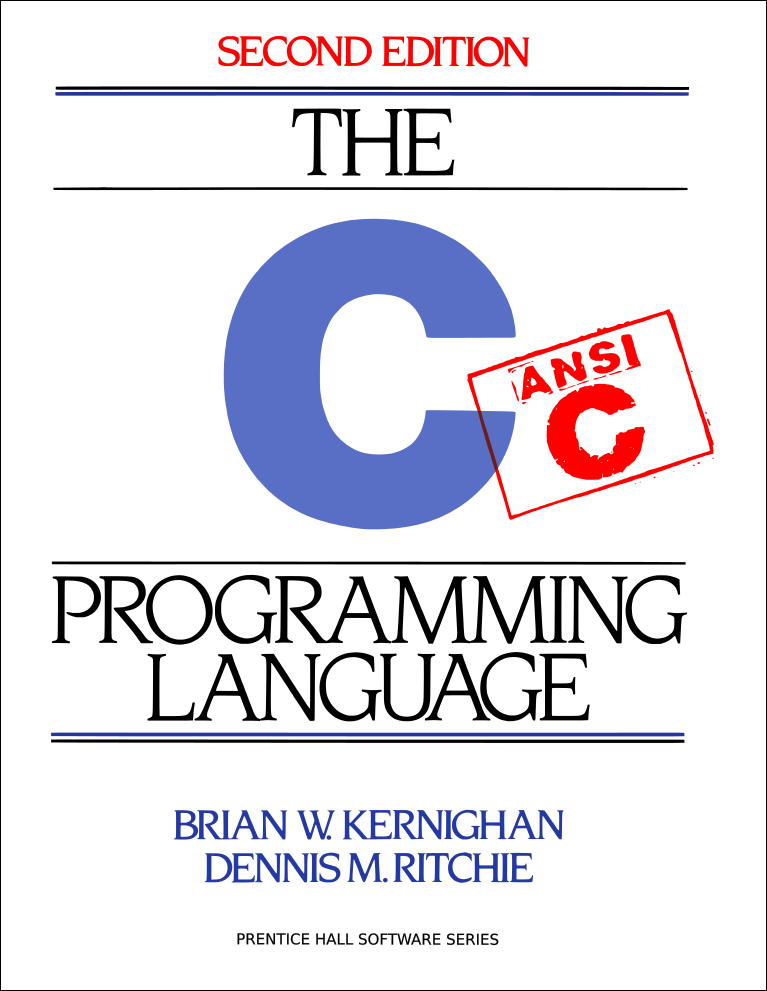
\includegraphics[width=\textwidth,keepaspectratio]{kandr}
      \caption{The bible.}
    \end{figure}
    \column{.6\textwidth}
    \begin{itemize}
    \item A C program consists of \textit{functions} and \textit{variables}.
      \pause
    \item A function contains \textit{statements} that specify the
      computing operations to be done.
      \pause
    \item Variables store values to be used during computation.
      \pause
    \item Normally you can name functions whatever you like, but every program
      must contain a function named \mintinline{text}{main}.
    \end{itemize}
  \end{columns}


\\

\end{frame}

\begin{frame}[fragile]
  \frametitle{Hello World}

\begin{minted}{c}
#include <stdio.h>

main() {
  printf("Hello, world!\n");
}
\end{minted}
\\
  \begin{itemize}
  \item In this example \mintinline{c}{printf} is a function that takes a
    \textit{character string} as its argument.
    \pause
  \item Copy the code above into an empty file \mintinline{text}{hello.c} in your
    \mintinline{text}{task1} directory (We'll help you find it.), and then from your
    terminal:
    \pause
  \end{itemize}
\bigskip
\begin{minted}[linenos=false]{text}
# cd ~/Desktop/bootcamp/task1
# gcc hello.c
# ./a.out
\end{minted}

\end{frame}

\begin{frame}[fragile]
  \frametitle{Prompts}

  From your terminal,
\begin{minted}[linenos=false]{text}
# cd ../task2
\end{minted}
\\
then open the file \mintinline{text}{prompt.c} in your text editor. You should
see the following:

\pause

\bigskip

\begin{minted}[fontsize=\footnotesize]{c}
#include <stdio.h>

main() {
  char name[40];
  printf("Enter your name:\n");

  // YOUR TASK: Prompt the user for their name say hello.

}
\end{minted}

\end{frame}

\begin{frame}[fragile]
  \frametitle{Prompts}

\begin{minted}[fontsize=\footnotesize]{c}
#include <stdio.h>

main() {
  char name[40];
  printf("Enter your name:\n");

  // YOUR TASK: Prompt the user for their name say hello.

}
\end{minted}

  \begin{itemize}
  \item For this task, we'll make use of a new function
\begin{minted}[linenos=false,bgcolor=lightgray,frame=none]{c}
scanf(char* format, ...)
\end{minted}
    \pause
  \item \mintinline{c}{scanf} reads characters from your terminal, interprets them
    according to the \mintinline{text}{format} you provide (consult your cheatsheet), and stores the
    results in the remaining arguments.
    \pause
  \item For example, to store a user-given string in \mintinline{text}{name},
\begin{minted}[linenos=false,frame=none]{c}
scanf("%s", name);
\end{minted}
  \end{itemize}

\end{frame}

\begin{frame}[fragile]
  \frametitle{Prompts}
\begin{minted}[fontsize=\footnotesize]{c}
#include <stdio.h>

main() {
  char name[40];
  printf("Enter your name:\n");

  // YOUR TASK: Prompt the user for their name say hello.

}
\end{minted}
  \begin{itemize}
  \item For example, to store a user-given string in \mintinline{text}{name},
\begin{minted}[linenos=false,frame=none]{c}
scanf("%s", name);
\end{minted}
  \item Similarly, \mintinline{c}{printf} can be given format specifiers in its
    first argument and will print the rest of its arguments accordingly.
\begin{minted}[linenos=false,frame=none]{c}
printf("Goodbye %s", name);
\end{minted}
    \pause
  \item Complete your task (Ask for your help if you're stuck!), and run your program.
  \end{itemize}
\end{frame}

\begin{frame}[fragile]
  \frametitle{Arguments}
  From your terminal,
\begin{minted}[linenos=false]{text}
# cd ../task3
\end{minted}
\\
  then open the file \mintinline{text}{arguments.c} in your text editor. You
  should see the following:
  \pause
\begin{minted}[fontsize=\footnotesize]{c}
#include <stdio.h>
#include <stdlib.h>

int main(int argc, char* argv[]) {
  if (argc < 3) {
    printf("Usage: %s <name> <integer>\n", argv[0]);
    return -1;
  }

  // YOUR TASK: Read the user's name and an integer
  // from command line arguments, then say hello
  // to the user as many times as given by the integer.

}
\end{minted}

\end{frame}

\begin{frame}[fragile]
  \frametitle{Arguments}

\begin{minted}{c}
int main(int argc, char* argv[]) {
  ...
}
\end{minted}

  \begin{itemize}
  \item Note that our \mintinline{c}{main} has grown a little.
    \pause
  \item The first \mintinline{c}{int} tells us that this function will return
    an integer.
    \pause
  \item \mintinline{c}{int argc} and \mintinline{c}{char* argv[]} are
    parameters to \mintinline{c}{main}.
    \pause
    \begin{itemize}
    \item \mintinline{c}{char* argv[]} is an array of strings containing all the
      arguments we'll pass when we run our program. (More on that later.)
      \pause
    \item \mintinline{c}{int argc} is an integer indicating the length of
      \mintinline{c}{argv} or the number of strings contained within.
    \end{itemize}
  \end{itemize}
\end{frame}

\begin{frame}[fragile]
  \frametitle{Arguments}
\begin{minted}{c}
int main(int argc, char* argv[]) {
  ...
}
\end{minted}

  \bigskip

  For example, if we invoke our program as follows:
\begin{minted}[linenos=false]{text}
# ./a.out CiComputerGirls 5
\end{minted}

  \pause

  \bigskip

  \begin{itemize}
  \item Then \mintinline{c}{argc} contains the integer 3.
    \pause
  \item \mintinline{c}{argv[0]} contains the string \mintinline{c}{"a.out"}.
    \pause
  \item \mintinline{c}{argv[1]} contains the string \mintinline{c}{"CiComputerGirls"}.
    \pause
  \item \mintinline{c}{argv[2]} contains the string \mintinline{c}{"5"}.
  \end{itemize}

\end{frame}

\begin{frame}[fragile]
  \frametitle{Arguments}

\begin{minted}[fontsize=\footnotesize]{c}
int main(int argc, char* argv[]) {
  if (argc < 3) {
    printf("Usage: %s <name> <integer>\n", argv[0]);
    exit(-1);
  }
  ...
}
\end{minted}

  \begin{itemize}
  \item In the given code, we examine \mintinline{c}{argc} in the condition of
    our if-statement to ensure our program was passed the correct number of
    arguments.
    \pause
  \item And if not, we print a helpful message and exit with an error code.
    \pause
  \item Note that our helpful message prints the value of
    \mintinline{c}{argv[0]}. The first string in \mintinline{c}{argv} will always
    be the name of your program.
  \end{itemize}

\end{frame}

\begin{frame}[fragile]
  \frametitle{Arguments}
\begin{minted}[fontsize=\footnotesize]{c}
int main(int argc, char* argv[]) {
  ...

  // YOUR TASK: Read the user's name and an integer
  // from command line arguments, then say hello
  // to the user as many times as given by the integer.

}

\end{minted}

\bigskip

To complete your task,

  \begin{itemize}
  \item Use the function \mintinline{c}{atoi} to convert the value of
    \mintinline{c}{argv[2]} into an \mintinline{c}{int}.
\begin{minted}[frame=none,linenos=false]{c}
int atoi(char* s)
\end{minted}
    \pause
  \item \mintinline{c}{atoi} converts the string \mintinline{c}{s} into an
    \mintinline{c}{int}. For example,
\begin{minted}[frame=none,linenos=false]{c}
int five = atoi("5");
\end{minted}
    \pause
  \item Then use a for- or while-loop to print your message as many times as needed.
  \end{itemize}

\end{frame}

\begin{frame}[fragile,fragile]
  \frametitle{Functions}

  From your terminal,
\begin{minted}[linenos=false]{text}
# cd ../task4
\end{minted}
  \\
  and open the file \mintinline{text}{functions.c} in your text editor.
  \pause

  \bigskip

\begin{minted}[fontsize=\footnotesize]{c}
#include <math.h>
#include <stdio.h>

// YOUR TASK: Implement the function get_population.

int get_population(int generation);

main() {
  ...
}
\end{minted}
\end{frame}

\begin{frame}[fragile]
  \frametitle{Functions}

  Each function definition has the form
  \bigskip

\begin{minted}[fontshape=it,fontfamily=lmtt,linenos=false]{text}
return-type function-name(argument declarations) {
  declarations and statements
}
\end{minted}

  \pause

  \bigskip

  Compare the above with our definition of the function \mintinline{c}{power} in
  \mintinline{text}{functions.c}. \pause

  \bigskip

\begin{minted}[fontsize=\footnotesize]{c}
int power(int base, int exp) {
  int result = 1;

  int i;
  for (i = 0; i < exp; i++)
    result *= base;

  return result;
}
\end{minted}

\end{frame}

\begin{frame}[fragile]
  \frametitle{Functions}

\begin{minted}[linenos=false]{c}
int get_population(int generation);
\end{minted}

  \bigskip

  \begin{itemize}
  \item Your implementation of \mintinline{c}{get_population} should conform to
    the specifications in the above declaration. \pause
    \begin{itemize}
    \item I.e., it should accept a single \mintinline{c}{int} as an argument and
      return an \mintinline{c}{int} to its caller. \pause
    \end{itemize}
  \item The rate at which your population grows is left up to you, but note that to
    work with our program shell, \mintinline{c}{get_population} should only
    increase with respect to its argument. \pause
    \begin{itemize}
    \item For a simple implementation consider that if each tribble can breed
      $2$ more tribbles, then after $3$ generations you have $2^3 = 8$ tribbles.
      \pause
    \item You can call \mintinline{c}{power} from within
      \mintinline{c}{get_population} to model this relationship.
    \end{itemize}
  \end{itemize}

\end{frame}

\begin{frame}[fragile]
  \frametitle{Pointers}

  Now \mintinline{text}{cd} into the \mintinline{text}{task5} directory and
  open \mintinline{text}{pointers.c} in your text editor.

  \pause

  \bigskip

\begin{minted}[fontsize=\footnotesize]{c}
#include <stdio.h>

main() {
  char *string1 = "This is the first string.";
  char *string2 = "This is the second string.";

  // YOUR TASK: Write a function `swap` that swaps the pointers
  // in its first and second arguments. Then invoke your function
  // with string1 and string2.

  printf("string1 = %s and string2 = %s\n", string1, string2);
}
\end{minted}

\end{frame}

\begin{frame}[fragile]
  \frametitle{Pointers}

\begin{minted}[fontsize=\footnotesize]{c}
main() {
  char *string1 = "This is the first string.";
  ...
}
\end{minted}

  \bigskip

  \begin{itemize}
  \item A \textit{pointer} is a variable that contains the address in memory of
    another variable. \pause
  \item C has two operators for dealing with pointers: \pause
    \begin{itemize}
    \item \mintinline{c}{*} is the \textit{dereferencing} operator. When applied
      to a pointer, it returns the value to which the pointer points. \pause
    \item \mintinline{c}{&} does the opposite of \mintinline{c}{*}. When applied
      to a variable, it returns the address at which the variable is stored.
    \end{itemize}
  \end{itemize}
\end{frame}

\begin{frame}[fragile]
  \frametitle{Pointers}

\begin{minted}[fontsize=\footnotesize]{c}
main() {
  char *string1 = "This is the first string.";
  ...
}
\end{minted}

  \begin{itemize}
  \item Note that the above code declares \mintinline{c}{string1} to be a
    pointer. It states that \mintinline{c}{string1} points to the location in
    memory of the beginning of the assigned string. \pause
  \item Now note that \mintinline{c}{*string1} is a \mintinline{c}{char}. The
    \mintinline{c}{*} applies the dereferencing operator to
    \mintinline{c}{string1}, returning the first value at the location to which
    pointer points. In this case, \mintinline{c}{'T'}.
  \end{itemize}

\end{frame}

\begin{frame}[fragile]
  \frametitle{Pointers}


  To write your swap function, you must be aware of one more caveat:
  \begin{itemize}
  \item As in most languages, C passes arguments to functions by value, so there
    is no way for a called function to alter a variable in the calling function.
    \pause
  \item Consider this function \mintinline{c}{swap} for swapping two integers:
  \end{itemize}

\begin{minted}[fontsize=\footnotesize]{c}
// WRONG!
void swap(int x, int y) {
  int temp;

  temp = x;
  x = y;
  y = temp;
}
\end{minted}
\pause
  \begin{itemize}
  \item Just like Java, this function will not work as intended. \pause
  \item \mintinline{c}{x} and \mintinline{c}{y} are swapped within the scope of our
    function \mintinline{c}{swap}, but since they were passed only by value to
    the function, they will not be swapped in any code that calls our \mintinline{c}{swap}.
  \end{itemize}
\end{frame}

\begin{frame}[fragile,fragile]
  \frametitle{Pointers}

  To obtain the desired effect, instead of writing a function that takes the
  values of the variables to be swapped, we write a function that takes the
  pointers to their values in memory:

\pause

\bigskip

\begin{minted}[fontsize=\footnotesize]{c}
void swap(int *px, int *py) {
  int temp;

  temp = *px;   // temp gets the value to which px points.
  *px = *py;    // The value at px gets the value at py.
  *py = temp;   // The value to which py points gets temp.
}
\end{minted}

\pause

\bigskip

We can invoke this \mintinline{c}{swap} like so:

\bigskip

\begin{minted}[fontsize=\footnotesize]{c}
int a = 5;
int b = 10;
swap(&a, &b);
// Now a == 10, and b == 5.
\end{minted}
\end{frame}

\begin{frame}[fragile]
  \frametitle{Pointers}

\begin{minted}[fontsize=\footnotesize]{c}
void swap(int *px, int *py) {
  int temp;

  temp = *px;   // temp gets the value to which px points.
  *px = *py;    // The value at px gets the value at py.
  *py = temp;   // The value to which py points gets temp.
}

int a = 5;
int b = 10;
swap(&a, &b);
// Now a == 10, and b == 5.
\end{minted}

  \begin{itemize}
  \item Note that to swap two \mintinline{c}{int} our function accepts two
    \mintinline{c}{int*}. \pause
  \item We use \mintinline{c}{&} to access the address at which our
    values are stored. In other words, to access \textit{pointers} to our
    variables \mintinline{c}{a} and \mintinline{c}{b}.
  \end{itemize}

\end{frame}

\begin{frame}[fragile]
  \frametitle{Pointers}

\begin{minted}[fontsize=\footnotesize]{c}
main() {
  char* string1 = "This is the first string.";
  char* string2 = "This is the second string.";

  // YOUR TASK: Write a function `swap` that swaps the pointers
  // in its first and second arguments. Then invoke your function
  // with string1 and string2.

  printf("string1 = %s and string2 = %s\n", string1, string2);
}
\end{minted}

  \begin{itemize}
  \item Since a string is already a pointer to a \mintinline{c}{char} (or a
    \mintinline{c}{char*}), your \mintinline{c}{swap} should take two pointers
    to \mintinline{c}{char} pointers (or two \mintinline{c}{char**}). \pause
  \item Implement \mintinline{c}{swap} and test your program. (And ask for help if
    you're stuck!)
  \end{itemize}

\end{frame}

\begin{frame}[fragile]
  \frametitle{Structs}

  Now \mintinline{text}{cd} into the \mintinline{text}{task6} directory and
  open \mintinline{text}{structs.c} in your text editor. \pause

\bigskip

\begin{minted}[fontsize=\footnotesize]{c}
typedef struct {
  char* name;
  int health;
  int* weapon_statuses; // An array whose elements indicate the
                        // status of each weapon.
                        // A value >= 100 indicates the weapon is
                        // ready to fire.
  int num_weapons;
} Spaceship;

// YOUR TASK: Implement charge_weapons and attack_ship.
void charge_weapons(Spaceship* ship);
void attack_ship(Spaceship* from, Spaceship* to);
\end{minted}
\end{frame}

\begin{frame}[fragile]
  \frametitle{Structs}

  \begin{columns}[c]
    \column{.4\textwidth}
\begin{minted}[fontsize=\footnotesize]{c}
typedef struct {
  char* name;
  int health;
  int* weapon_statuses;
  int num_weapons;
} Spaceship;
\end{minted}
    \column{.6\textwidth}
    \begin{itemize}
    \item A struct is simply a collection of one or more variables, grouped
      together under a single name. \pause
    \item As defined, our \mintinline{c}{Spaceship} struct contains the variables
      \mintinline{c}{name}, \mintinline{c}{health},
      \mintinline{c}{weapon_statuses}, and \mintinline{c}{num_weapons}.
    \end{itemize}
  \end{columns}

\end{frame}

\begin{frame}[fragile,fragile]
  \frametitle{Structs}
  C defines two operators for dealing with structs. A member of a struct is
  referred to with the \mintinline[escapeinside=||]{c}{|\strut|.} operator, as shown below:

\bigskip

\begin{minted}{c}
Spaceship starship = ...
printf("The name of our ship is %s", starship.name);
\end{minted}
\pause

\bigskip

However as you can see from the function declarations in
\mintinline{text}{structs.c}, dealing with a pointer to a struct instead of
structs themselves is quite common. To refer to a member of a struct from a
pointer, use the \mintinline[escapeinside=||]{c}{|\strut|->} operator.

\bigskip

\begin{minted}{c}
Spaceship *ship = ...
printf("The name of our ship is %s", ship->name);
\end{minted}

\end{frame}

\begin{frame}[fragile]
  \frametitle{Structs}

\begin{minted}[fontsize=\footnotesize]{c}
typedef struct {
  char* name;
  int health;
  int* weapon_statuses; // An array whose elements indicate the
                        // value of each weapon.
                        // A value >= 100 indicates the weapon is
                        // ready to fire.
  int num_weapons;
} Spaceship;

// YOUR TASK: Implement charge_weapons and attack_ship.
void charge_weapons(Spaceship* ship);
void attack_ship(Spaceship* from, Spaceship* to);
\end{minted}

  \bigskip

  \begin{itemize}
  \item Implement the two functions and test your program.
  \item Note that to \mintinline{c}{weapon_statuses} is an array, so to access an
    element you apply an index like so: \mintinline{c}{ship->weapon_statuses[0]}.
  \end{itemize}

\end{frame}

\begin{frame}[fragile]
  \frametitle{Headers}

  Now \mintinline{text}{cd} into the \mintinline{text}{task7} directory and
  open \mintinline{text}{headers.c} in your text editor. \pause

  You'll find an incomplete implementation of a linked-list struct.

\bigskip

\begin{minted}[fontsize=\footnotesize]{c}
// headers.c

// YOUR TASK: Write a header file for the linked-list
// implementation below, exposing list_append(), list_prepend(),
// and the struct itself.

#include "headers.h"

struct List {
  void* data;
  struct List* next;
};

...
\end{minted}

\end{frame}

\begin{frame}
  \frametitle{Headers}

  \begin{itemize}
  \item Think of header files as the public documentation of any program or
    library you write. \pause
  \item I.e., declarations for any functions we would consider ``public'' in an
    OOP language go in our header file. Declarations of functions we would
    consider ``private'' can remain in our source file. \pause
  \item Anyone using the provided linked-list library would probably want the
    ability to declare instances of \mintinline{c}{struct List} and append and
    prepend to it, so we declare those in the header.
  \end{itemize}
\end{frame}

\begin{frame}
  \frametitle{Further Work}

  If you'd like to continue your studies, please consider:

  \begin{itemize}
  \item Procuring a copy of \emph{The C Programming Language} by Kernighan and
    Ritchie. \pause
  \item Visiting the C tutorials on Lynda.com, free to all students at CSUCI.
    \pause
  \item Familiarizing yourself with the command line through online courses such
    as those at Codecademy.com.
  \end{itemize}
\end{frame}

\end{document}
